\section{Object3DContainer Class Reference}
\label{classObject3DContainer}\index{Object3DContainer@{Object3DContainer}}
{\tt \#include $<$object3dcontainer.h$>$}

Inheritance diagram for Object3DContainer::\begin{figure}[H]
\begin{center}
\leavevmode
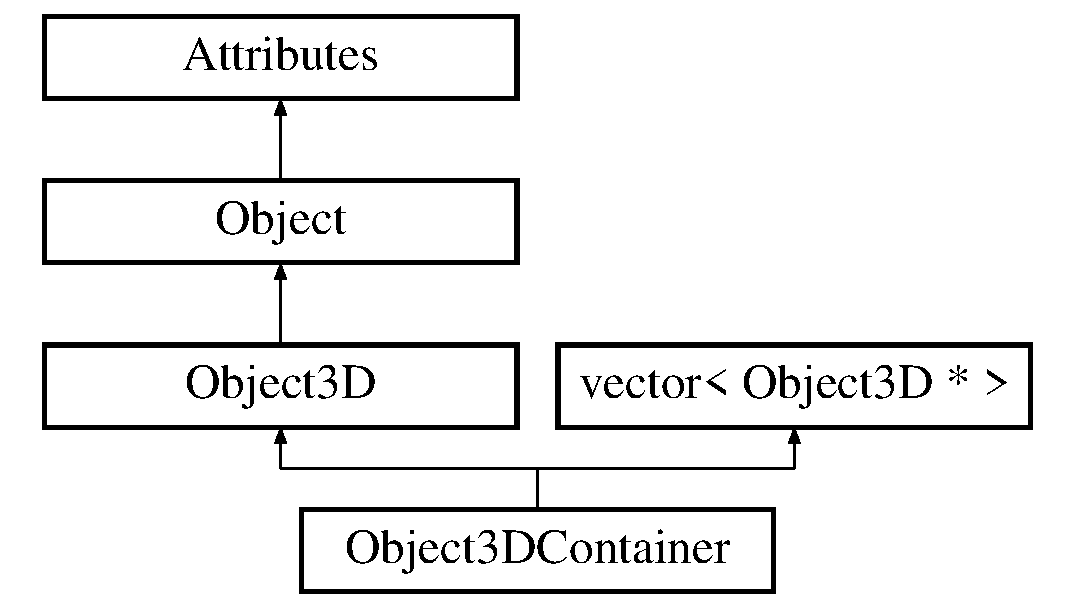
\includegraphics[height=4cm]{classObject3DContainer}
\end{center}
\end{figure}
\subsection*{Public Methods}
\begin{CompactItemize}
\item 
std::pair$<$ double, double $>$ {\bf get\-Depth\-Range} ()
\item 
void {\bf render} ({\bf Figure} $\ast$, double x\-Offset, double y\-Offset, double scale, double distance, double min\-Range=0, double max\-Range=0, int min\-Fig\-Depth=0, int max\-Fig\-Depth=999)
\item 
void {\bf apply\-Matrix} ({\bf Matrix}$<$ double $>$ $\ast$m)
\item 
void {\bf translate} ({\bf Coordinate3D} $\ast$)
\end{CompactItemize}


\subsection{Member Function Documentation}
\index{Object3DContainer@{Object3DContainer}!applyMatrix@{applyMatrix}}
\index{applyMatrix@{applyMatrix}!Object3DContainer@{Object3DContainer}}
\subsubsection{\setlength{\rightskip}{0pt plus 5cm}void Object3DContainer::apply\-Matrix ({\bf Matrix}$<$ double $>$ $\ast$ {\em m})\hspace{0.3cm}{\tt  [virtual]}}\label{classObject3DContainer_a2}




Implements {\bf Object3D} {\rm (p.\,\pageref{classObject3D_a2})}.\index{Object3DContainer@{Object3DContainer}!getDepthRange@{getDepthRange}}
\index{getDepthRange@{getDepthRange}!Object3DContainer@{Object3DContainer}}
\subsubsection{\setlength{\rightskip}{0pt plus 5cm}std::pair$<$ double, double $>$ Object3DContainer::get\-Depth\-Range ()\hspace{0.3cm}{\tt  [virtual]}}\label{classObject3DContainer_a0}




Implements {\bf Object3D} {\rm (p.\,\pageref{classObject3D_a0})}.\index{Object3DContainer@{Object3DContainer}!render@{render}}
\index{render@{render}!Object3DContainer@{Object3DContainer}}
\subsubsection{\setlength{\rightskip}{0pt plus 5cm}void Object3DContainer::render ({\bf Figure} $\ast$, double {\em x\-Offset}, double {\em y\-Offset}, double {\em scale}, double {\em distance}, double {\em min\-Range} = 0, double {\em max\-Range} = 0, int {\em min\-Fig\-Depth} = 0, int {\em max\-Fig\-Depth} = 999)\hspace{0.3cm}{\tt  [virtual]}}\label{classObject3DContainer_a1}




Implements {\bf Object3D} {\rm (p.\,\pageref{classObject3D_a1})}.\index{Object3DContainer@{Object3DContainer}!translate@{translate}}
\index{translate@{translate}!Object3DContainer@{Object3DContainer}}
\subsubsection{\setlength{\rightskip}{0pt plus 5cm}void Object3DContainer::translate ({\bf Coordinate3D} $\ast$)\hspace{0.3cm}{\tt  [virtual]}}\label{classObject3DContainer_a3}




Implements {\bf Object3D} {\rm (p.\,\pageref{classObject3D_a3})}.

The documentation for this class was generated from the following files:\begin{CompactItemize}
\item 
{\bf object3dcontainer.h}\item 
{\bf object3dcontainer.cpp}\end{CompactItemize}
